\chapter{Product Deployment Architecture}

The VoiceScore system is designed as an interactive, consumer-facing application. To achieve low latency, high availability, and cost-effective scalability, the architecture is split across multiple specialized hosting platforms.

\section{Split Architecture Design}
The system architecture isolates the heavy machine learning inference from the lightweight user interface rendering.

\begin{figure}[h]
    \centering
    \begin{tikzpicture}[
        box/.style={draw=blue!60!black, rectangle, minimum width=4.8cm, minimum height=1.2cm, align=center, rounded corners=4pt, font=\small, thick},
        arrow/.style={->, >=Stealth, thick, color=blue!80!black}
    ]
        % Top Level: Vercel Frontend
        \node[box, fill=purple!10] (vercel) at (0, 4.2) {\textbf{Vercel Deployment} \\ (Next.js Web Frontend)};
        
        % Middle Level: FastAPI Backend
        \node[box, fill=cyan!10] (hf) at (0, 1.8) {\textbf{Hugging Face Spaces} \\ (FastAPI Docker Backend)};
        
        % Bottom Level: Inference Model & Database
        \node[box, fill=orange!10] (model) at (-3.4, -0.6) {\textbf{nptel-asr-phoneme-v3} \\ (Wav2Vec2 Inference Engine)};
        \node[box, fill=green!10] (db) at (3.4, -0.6) {\textbf{Supabase DB} \\ (PostgreSQL \& Prisma ORM)};
        
        % Connections
        \draw[arrow] (vercel) -- node[right, font=\tiny\bfseries, color=black] {HTTPS / REST API} (hf);
        \draw[arrow] (hf) -- node[above left, font=\tiny\bfseries, color=black, align=right] {Acoustic\\Inference} (model);
        \draw[arrow] (hf) -- node[above right, font=\tiny\bfseries, color=black, align=left] {Database\\Queries} (db);
    \end{tikzpicture}
    \caption{VoiceScore Split Architecture Layout}
    \label{fig:architecture}
\end{figure}

\subsection{Frontend: Vercel (Next.js)}
The frontend is built using React and Next.js, hosted on Vercel for fast, edge-cached content delivery (\url{https://pronounhelp.vercel.app/}). The User Interface (UI) embraces a futuristic "dark glassmorphic" aesthetic to reduce eye strain and provide a premium feel. 

\begin{figure}[h]
    \centering
    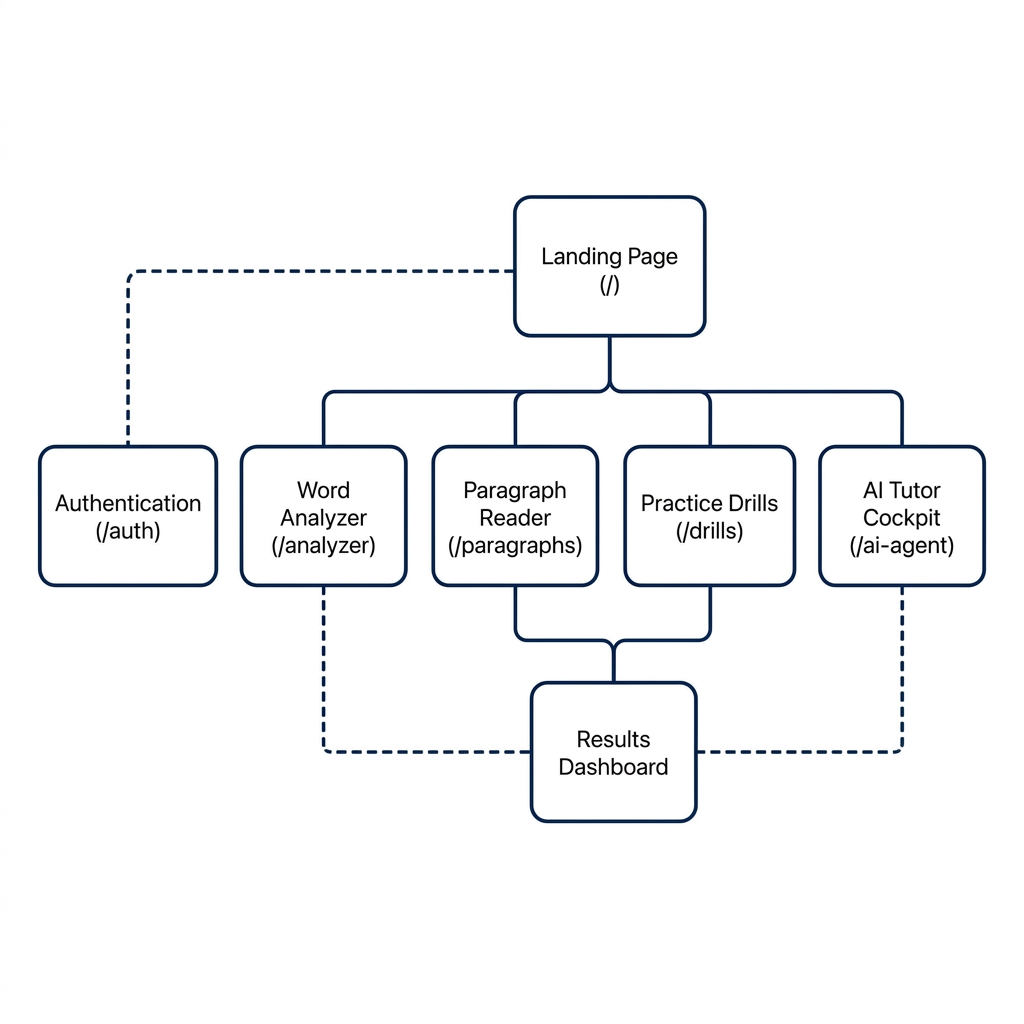
\includegraphics[width=\textwidth]{../docs/product_navigation.png}
    \caption{Product Page and Flow Navigation Map}
    \label{fig:product_navigation}
\end{figure}

Key frontend components include:
\begin{itemize}
    \item \textbf{Word \& Paragraph Analyzer:} Interactive heatmaps that color-code words based on pronunciation accuracy (Green = Correct, Orange = Minor Error, Red = Critical Error). Hovering over words reveals glassmorphic tooltips displaying a side-by-side token comparison to highlight insertions, deletions, or substitutions.
    \item \textbf{Audio Visualization:} A custom HTML5 Web Audio API visualizer renders real-time waveforms as the user speaks into the microphone.
\end{itemize}

\subsection{Backend: Hugging Face Spaces (FastAPI)}
The backend API is deployed on Hugging Face Spaces via Docker SDK (\url{https://mihirrpatil-asr.hf.space}). A custom Dockerfile utilizing a slim Python 3.10 base image installs essential audio processing libraries (\texttt{ffmpeg}, \texttt{libsndfile1}) alongside the CPU-only distribution of PyTorch to minimize image size. The backend handles the computationally expensive Wav2Vec2 inference (\url{https://huggingface.co/MihirRPatil/nptel-asr-phoneme-v3}) and forced alignment tasks. 

Furthermore, to ensure cross-browser compatibility (as Chrome, Safari, and Firefox produce different audio codecs like WebM or Opus), the backend employs a system-level FFmpeg pipeline to transcode all incoming audio buffers into 16kHz mono WAV format before passing them to the acoustic model.

\subsection{Database: Supabase (PostgreSQL)}
User history, performance logs, and spaced repetition review schedules are persisted in a Supabase PostgreSQL database. The backend interfaces with the database via the Prisma Object-Relational Mapper (ORM), utilizing connection pooling to handle concurrent analytical requests.

\begin{table}[h]
    \centering
    \small
    \caption{Live Production Endpoints and Repository Locations}
    \label{tab:deployed_links}
    \begin{tabular}{p{4.2cm} p{3.8cm} p{6.5cm}}
        \toprule
        \textbf{Component Layer} & \textbf{Hosting Platform} & \textbf{Production URL / Resource} \\
        \midrule
        Web Frontend & Vercel & \url{https://pronounhelp.vercel.app/} \\
        Inference Backend API & Hugging Face Spaces & \url{https://mihirrpatil-asr.hf.space} \\
        Model Weights & Hugging Face Hub & \url{https://huggingface.co/MihirRPatil/nptel-asr-phoneme-v3} \\
        Database Storage & Supabase Cloud & Managed PostgreSQL Instance \\
        \bottomrule
    \end{tabular}
\end{table}

\section{AI Tutor Integration (OpenRouter)}
A standout feature of the product is the "AI Tutor Cabin" (\texttt{/ai-agent}). To build conversational fluency, users require interactive practice rather than merely reading static text. 

The backend integrates with OpenRouter's API to access advanced Large Language Models (LLMs). The system employs a robust fallback chain, initially querying \texttt{gemma-2-9b-it} (\texttt{google/}\allowbreak\texttt{gemma-2-9b-it:free}) for low latency, and falling back to \texttt{llama-3.3-70b-instruct} (\texttt{meta-llama/}\allowbreak\texttt{llama-3.3-70b-instruct:free}) if rate limits are hit. 

The AI Tutor presents users with three contextual response options (e.g., Professional, Casual, Inquisitive). The user reads their chosen response aloud, receiving real-time GoP scoring. The LLM then generates a conversational reply, which is synthesized into speech using integrated Text-to-Speech (TTS) endpoints, creating a fully immersive, stress-free spoken English practice environment.
